%\pagestyle{scrheadings}
%\ohead{Kapitel 2: Theoretischer Hintergrund }

\section{Theoretischer Hintergrund}
Dadurch bedingt, das diese Arbeit sich an vielen Konzepten aus der Signaltheorie, Elektrotechnik, Informatik und Mathematik bedient, ist es sinnvoll vorab einige Begriffe und Konzepte zu definieren und zu erläutern. Aus diesem Grund, werden im Folgenden das I²C Protokoll, das Nyquist-Frequenz Theorem, die Grundlagen von Neuronalen Netzen sowie die verwendete Software näher erläutert. 

\subsection{Hybrid-Buck-Wandler}
Bei dem Buck-Wandler handelt es sich um einen DC-DC Wandler, das bedeutet, dieser Wandler nimmt eine Gleichstrom Eingangsspannung von 15 bis 40 Volt entgegen und setzt diese herunter auf eine Gleichstrom Ausgangsspannung von zwölf Volt. In Abb. 1 ist besagter Wandler zu erkennen. \hl{Unten rechts in der Abbildung ist der Eingang zu sehen, oben rechts der Ausgang und links mittig ist die I²C Schnittstelle angebracht}. Des Weiteren ist der hier verwendete Wandler auf einen Stromfluss von zehn Ampere limitiert, was bedeutet, dass die maximale Leistung am Ausgang des Wandlers 120 Watt beträgt. Es bedeutet ebenfalls, dass, wenn der Strom zehn Ampere übersteigt, die Ausgangsspannung gedrosselt wird. Für den weiteren Verlauf der Arbeit wird für den vorgestellten Hybrid DC-DC Wandler immer der simplere Begriff "Wandler" verwendet.
Der Wandler besitzt ebenfalls eine I²C Schnittstelle, aus welcher Ausgangsspannung, Eingangsspannung, Ausgangsstrom und Temperatur des Boards gemessen und ausgelesen werden können. Die Datenleitungen des I²C Busses sind bereits auf dem Wandler mit Pull-Up Widerständen ausgestattet, wodurch die Leitungen im unbenutzten Zustand auf fünf Volt gesetzt sind. Dadurch müssen keine externen Pull-Up Widerstände an die Leitungen angeschlossen werden.

\begin{figure}[H]
    \centering
    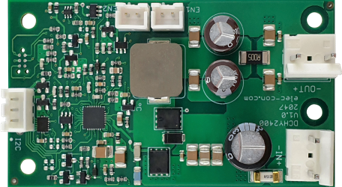
\includegraphics[height= 7cm, width = \textwidth]{Pictures/Wandler.png}
    \caption{Verwendeter Hybrid DC-DC Wandler}
\end{figure}

\subsection{I2C}
I2C steht für Inter-Integrated Circuit und wurde von Philips Semiconductors im Jahr 1982 entwickelt. Es handelt sich dabei um einen seriellen Datenbus im Master-Slave Stil. Dieses Protokoll besitzt insgesamt vier Leitungen, von denen jeweils eine für die Versorgungsspannung und eine als Ground verwendet wird. Des Weiteren werden zwei Leitungen für den Datenaustausch verwendet, davon ist ein Kanal explizit für die Daten (Serial Data) und der andere Kanal für den Takt (Serial Clock) vorgesehen. Der Takt des I²C Protkolls ist dabei auf Werte zwischen 100 KHz (standard mode) und 3.2 MHz (high speed) spezifiziert. 
\\
In Abb. 2 sind die genannten Master und Slave Komponenten zu erkennen. Der Master gibt allen Slaves vor, was sie zu senden haben, und wie schnell diese es tun sollen. Des Weiteren ist zu erkennen, das die beiden Leitungen SDA und SCL an einem Pull-Up Widerstand angeschlossen sind. Dieser dient dazu, die Leitungen, wenn weder Master noch Slave senden, auf die Versorgungsspannung zu schalten, sodass keine undefinierten Zustände entstehen und die Leitung im unbenutzten Zustand eine logische eins besitzt, also aktiv ist. Die Kommunikation erfolgt durch Adressen, so besitzt jeder Sensor oder Mikrocontroller eine I2C Adresse, über die ein Master auf diese zugreifen kann. Das auslesen der Daten eines Slaves erfolgt per Registeradressen, so hat beispielsweise ein beliebiger I²C fähiger Sensor ein Register, in dem bestimmte Werte gespeichert sind. In dieser Arbeit handelt es sich bei dem I2C Slave um einen Mikrocontroller auf dem Buck-Wandler. Als Master können sowohl ein PICkit Serial Analyzer als auch ein Raspberry Pi fungieren.


\begin{figure}[H]
    \centering
    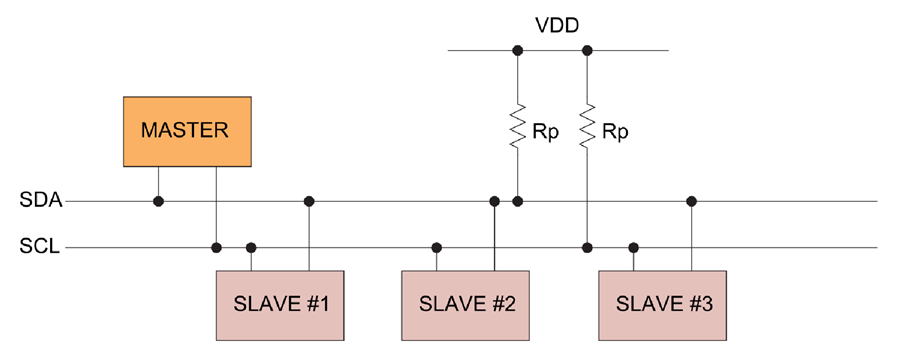
\includegraphics[height= 6cm, width = \textwidth]{Pictures/I2C_Bus.png}
    \caption{I2C Bus Beispiel }
\end{figure}

Die o. g. Kommunikation des I²C Protokolls erfolgt per Datenframes. Diese beinhalten Informationen bezüglich Start- und Stopbedingungen, Adressen sowie gesendete Daten. In Abb. \hl{x} ist die Struktur eines I²C Datenframes visualisiert. Dieses beginnt immer mit einer Startbedingung. Eine Startbedingung entspricht einem Wechsel des SDA Signals von High auf Low, während SCL High ist. Sobald SDA auf Low gesetzt wurde, wird auch SCL auf Low gesetzt. Darauf folgt die Adresse des Gerätes, mit dem kommuniziert werden soll, welche zwischen sieben und zehn Bit lang ist. Nach der Adresse folgt ein einzelnes Bit des Senders um zu signalisieren, ob geschrieben oder gelesen werden soll. Danach kommt vom Empfänger ein acknowledge (ACK) oder not-acknowledged (NACK) zurück, je nachdem, ob die anfrage erfolgreich war oder nicht. Im Falle eine nicht erfolgreichen Anfrage (NACK) bricht der Master die Kommunikation ab. Sollte die Anfrage erfolgreich gewesen sein, folgt darauf hin ein oder mehrere Datenbytes mitsamt einem ACK bzw. NACK wenn die Daten erfolgreich empfangen wurden. Sobald die Kommunikation abgeschlossen ist, wird diese mit einer Stop-Condition beendet. Die Stop-Condition ist das Pendant zu der Start-Condition, da diese durch das setzen des SCL Buses auf High und dem darauffolgenden setzen des SDA Buses auf High durchgeführt wird.


\begin{figure}[H]
    \centering
    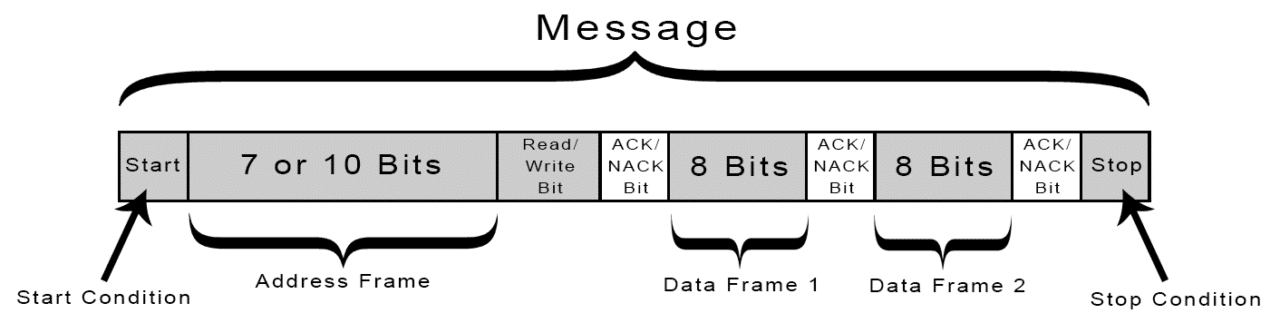
\includegraphics[height= 6cm, width = \textwidth]{Pictures/i2c_adr.png}
    \caption{Struktur eines I²C Datenframes}
\end{figure}



\subsection{Nyquist Frequenz Theorem}

Das Nyquist Frequenz Theorem ist eine fundamentale Aussage über das Verhältnis von Signalfrequenz und Abtastfrequenz bei der Digitalisierung von Analogen Signalen. Für diesen Sachverhalt existiert die Gleichung \hl{Nr. X}. Diese Gleichung sagt aus, das die maximale Signalfrequenz, welche ohne Verzerrungen, dem sog. "Alias-Effekt", dargestellt werden kann, der Hälfte der Abtastrate entspricht. 


\begin{equation}
\label{Nyquist}
f\textsubscript{nyquist} = 1/2 * f\textsubscript{abtastrate}
\end{equation}


Um dies zu verdeutlichen, sind in Abb. \hl{X} zwei Signale zu erkennen. Das ursprüngliche Signale (in blau aufgetragen) und das zweite Signal (rot aufgetragen), welches durch Abtastung generiert wurde. Bei dem ursprünglichen Signal handelt es sich um eine Sinuswelle mit einer Frequenz von \hl{100 Hz. Die Abtastrate beträgt ebenfalls 100 Hz}. Sobald die Formel \hl{x} auf diesen Sachverhalt angewendet wird, wird klar, dass die maximale Signalfrequenz bei \hl{100 Hz * 1/2 = 50 Hz liegt}, die tatsächliche Frequenz jedoch bei 100 Hz. Daraus resultiert der Alias Effekt, welcher im roten Signal zu erkennen ist.

\begin{figure}[H]
    \centering
    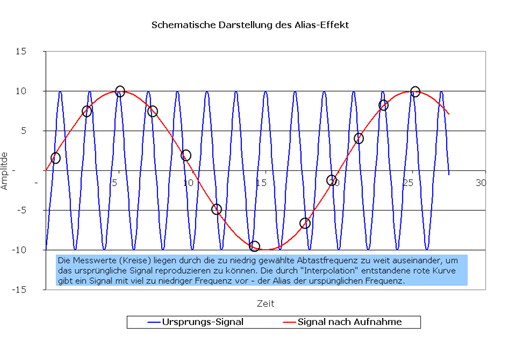
\includegraphics[height= 6cm, width = \textwidth]{Pictures/Alias.png}
    \caption{Beispiel des Alias Effekt}
\end{figure}

\subsection{Normalisierung der Daten}
Im bereich des Maschine Learning und Data Science ist es gängige Praxis vorhandene Daten, welche unterschiedliche Skalierungen besitzen zu Normalisieren. Normalisieren bedeutet, dass Daten insoweit verändert werden, dass sie in einem bestimmten Wertebereich dargestellt werden können. Diesbezüglich existieren mehrere Rechenmethoden, wie z. B. die z-Transformation oder feature scaling. Im Folgenden soll der Algorithmus des feature scaling näher erläutert werden. 


\begin{figure}[H]
    \centering
    \subfloat[\centering Normalisierte Daten]{{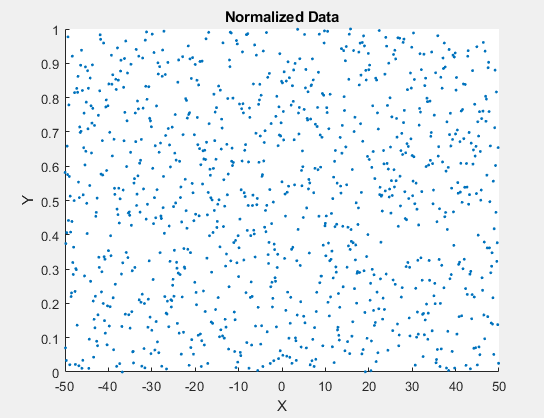
\includegraphics[width=6cm]{Pictures/Norm.png} }}%
    \qquad
    \subfloat[\centering Daten vor der Normalisierung]{{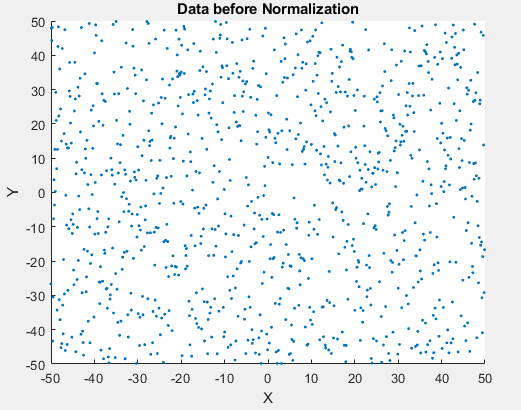
\includegraphics[width=6cm]{Pictures/NotNorm.png} }}%
    \caption{Normalisierung von Daten}%
    \label{Normalisierung}%
\end{figure}

In Abb. \hl{x} (b) ist ein Datensatz mit tausend zufällig generierten Werten zwischen -50 und +50 zu erkennen. Durch das anwenden der Gleichung \hl{x} für Normalisierte Daten, wobei max(x) und min(x) jeweils die maximalen, bzw. minimalen Datenwerte des Datensatzes sind, wird der Datensatz auf Werte zwischen null und eins angepasst. Dies hat für Maschine Learning Anwendungen den Vorteil, dass die Trainingszeit verkürzt werden kann und die Chance verringert wird, in lokalen Minima der Kostenfunktion \hl{"stecken zu bleiben"}. 

\begin{equation}
\label{Feature Scaling}
X' = \frac{X + max(X)}{max(X) - min(X)}
\end{equation}



\subsection{Neuronale Netze}

Zur Durchführung einiger simpler Testfälle unter den Punkten 3.2.1 und 3.2.2 ist es notwendig, eines der Grundlegenden Konzepte von Machine Learning zu erläutern: das Neuronale Netz.
Neuronale Netze gehören zur Maschine Learning Kategorie des "supervised learning". Beim supervised learning werden die Parameter eines neuronalen Netzes anhand der Eingabedaten (Input) und bereits definierten Lösungen (Output) daraufhin optimiert, bei gegebenen Input eine passende Lösungsstrategie für den bereits definierten Output zu finden. 


\begin{figure}[H]
    \centering
    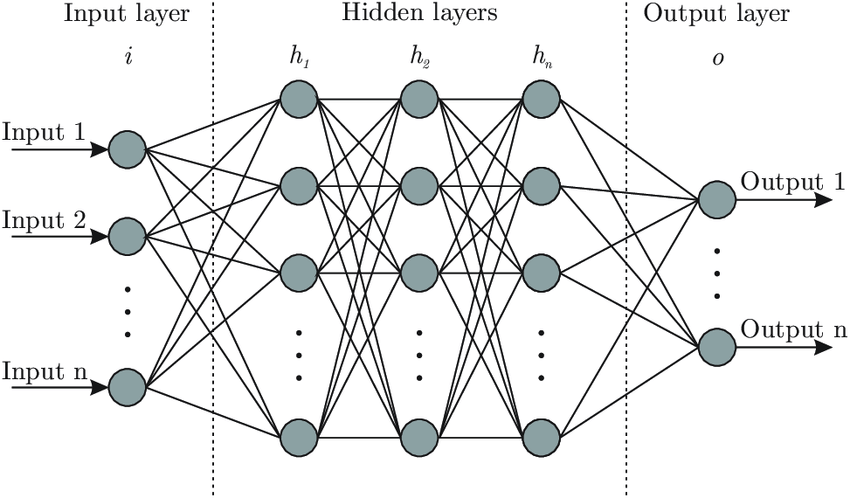
\includegraphics[height= 7cm, width = \textwidth]{Pictures/NN_Concept.png}
    \caption{Beispiel eines Neuronalen Netzes:}
\end{figure}


In Abb. 2 erkennt man eine Abbildung der Architektur eines möglichen neuronalen Netzes. Dieses ist aufgeteilt in mehrere Schichten: Input layer,hidden layer und Output layer. Das Input layer nimmt die Daten auf, welche verarbeitet werden müssen. Diese Daten können von verschiedener Art sein, so können es z. B. Pixeldaten eins Bildes sein, oder der Zeitverlauf eines Signals. Im hidden layer werden die Daten durch diverse mathematische Operationen verarbeitet, um im Output layer Aussagen über die Input Daten machen zu können, d. h. um die Input Daten zu klassifizieren.
\\
Neben den einzelnen Schichten ist zu erkennen, dass es mehrere Knoten gibt, welche untereinander durch Kanten vollvermascht sind. Die Knoten werden im Allgemeinen "Neuronen" genannt und sie besitzen einen numerischen Wert, welcher bestimmt, wie "aktiv" sie sind. Die Kanten, die die Neuronen verbinden, werden "weights\" oder Gewichtungen genannt. Die Gewichtungen sind dabei die Hauptparameter eines Neuronalen Netzes.

\\
Bei Neuronalen Netzen wird zwischen zwei Algorithmen unterschieden, dem Feedforward Algorithmus, welcher bei gegebenen Input Daten und Gewichtungen einen bestimmten Output liefert. Und dem Backpropagation Algorithmus, welcher bei gegebenem Input und Output neue Gewichtungen für das Neuronale Netz berechnet. Im Folgenden werden beide Algorithmen näher erläutert. 



\subsubsection{Feedforward Algorithmus}
\begin{figure}[H]
    \centering
    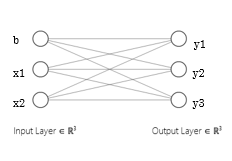
\includegraphics[height= 6cm, width = 6cm]{Pictures/FF.png}
    \caption{Konzept des Feedforward Algorithmus }
    
\end{figure}


\hl{Abb. X} zeigt ein vereinfachtes Neuronales Netzt mit zwei Schichten. Das Input layer nimmt zwei Eingangswerte entgegen und verrechnet diese per Matrixmultiplikation mit den Gewichtungen, wie in \hl{Gleichung X dargestellt}. Nach dieser Matrixmultiplikation entsteht ein neuer Vektor mit der gleichen Dimension wie der Output layer. Zu diesem Vektor wird noch der sog. "Bias" addiert. Der Bias dient als feste Skalierung dazu, ein Neuron gezielt mehr, bzw. weniger Aktiv zu machen, das bedeutet mathematisch, dass der numerische Wert gezielt gesteigert bzw. verringert wird. Nachdem der Input mit den Gewichtungen und dem Bias verrechnet wurde, wird auf das Ergebnis eine Aktivierungsfunktion angewendet. Eine Aktivierungsfunktion dient dazu zu bestimmen, wie "aktiv" ein Neuron ist. Es existieren mehrere Aktivierungsfunktionen. So zeigen Abbildungen 4 und 5 zwei Mögliche Funktionen. 

\begin{equation}
\label{Feedforwards}
    
          A\Bigg(
         \begin{bmatrix}
           w_{10}  w_{11} \\     
           w_{20}  w_{21} \\           
           w_{30} w_{31}
          \end{bmatrix}
          \begin{bmatrix}
           x_{1} \\
           x_{2} \\
         \end{bmatrix}
         + 
         \begin{bmatrix}
           b_{1} \\
           b_{2} \\
           b_{3} \\
         \end{bmatrix}
            \Bigg)
          =
          \begin{bmatrix}
           y_{1} \\
           y_{2} \\
     
           y_{3}
         \end{bmatrix}
         
\end{equation}



Die Formel für die Sigmoid Funktion: 

\begin{equation}
\label{Sigmoid}
s(z) = \frac{1}{1+e^{-z}}
\end{equation}


In Abb. 6 sind zwei existierende Aktivierungsfunktionen zu sehen, der Sigmoid die ReLu Funktion. Die ReLu Funktion gehört zu den beliebtesten Aktivierungsfunktionen, da diese Linearität gewährleistet. Wenn der Eingang der Funktion kleiner oder gleich 0 ist, dann ist der Ausgang immer 0. Für Werte größer als 0, ist der Output immer die Identitätsfunktion. Diese Funktion hat den Vorteil, dass sie negative Werte ignoriert, und positive Werte unverändert durchlässt. Des Weiteren ist zu erkennen, dass diese Funktion an der Stelle x = 0 nicht differenzierbar ist, da dort ein Knick vorzufinden ist.

Neben der ReLu Funktion ist aber auch der Sigmoid weitläufig bekannt. Dieser unterscheidet sich von der ReLu Funktion dadurch, dass diese nichtlinear (siehe Gleichung \hl{3} ist und sowohl negative als auch positive Ausgangswerte erlaubt. Im allgemeinen ist die ReLu Funktion \hl{bevorzugt} zu verwenden, da diese Linearität gewährleistet


\[ y = \left\{ \begin{array}{ll}
         0 & \mbox{if $x <= 0$}\\
	        x & \mbox{if $x > 0$}\end{array} \right. \] 
	        
	        
\begin{figure}%
    \centering
    \subfloat[\centering Sigmoid]{{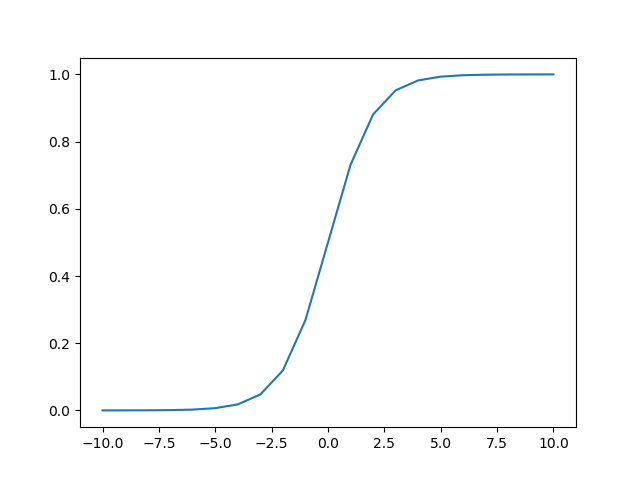
\includegraphics[width=6cm]{Pictures/Sigmoid.png} }}%
    \qquad
    \subfloat[\centering Rectified Linear Unit]{{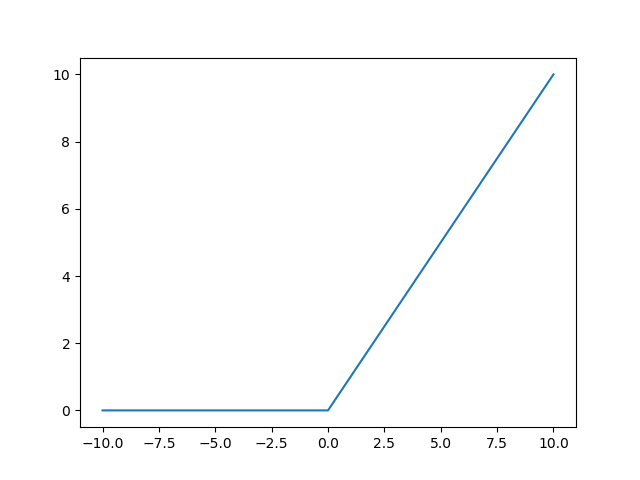
\includegraphics[width=6cm]{Pictures/Relu.png} }}%
    \caption{zwei mögliche Aktivierungsfunktionen}%
    \label{Aktivierungsfunktionen}%
\end{figure}



\subsubsection{Backpropagation Algorithmus}
Der zweite, wichtig Algorithmus für ein Neuronales Netz ist der Backpropagation Algorithmus. Dieser sorgt dafür, dass die vorher erwähnten Gewichtungen an die Input-Output Datenpaare angepasst werden, sodass später korrekte Vorhersagen allein durch die Input Daten gemacht werden können. \hl{Dies funktioniert konzeptionell so, dass der Fehler, welcher zwischen den tatsächlichen und den berechneten Ausgangsdaten entsteht, von den Output Knoten zurückpropagiert wird, so dass für jeden davorgehenden Knoten ebenfalls ein Fehler berechnet werden kann.} Für diesen Algorithmus muss eine neue Funktion eingeführt werden: Die Verlustfunktion. Die Verlustfunktion, wie sie als Gleichung \hl{x} dargestellt ist, ist eine Funktion in Abhängigkeit der Gewichtungen und sie berechnet den Fehler von den vorhergesagten Daten und den tatsächlichen Daten. Es existieren mehrere Möglichkeiten den Fehler zu berechnen, \hl{die Cross Entropy Methode ist jedoch mehr oder weniger standard}. In der Gleichung wird zwei mal summiert. die erste Summe berechnet die Fehler in den einzelnen Output Neuronen. So ist K z . B. gleich 3, falls 3 Output Neuronen existieren. In diesem Fall wird für jedes Neuron der vorhergesagte Wert und der tatsächliche Wert verglichen. Die Zweite Summe summiert die berechnete Summe des \hl{Neuronen vergleichs} über alle Datensätze, die in das Neuronale Netz eingespeist wurden. Darauffolgend wird das Ergebnis durch die Anzahl der Datensätze geteilt, um den durchschnittlichen Verlust zu berechnen


\begin{equation}
\label{Cross Entropy Loss}
J(\theta) = -\frac{1}{m} \sum_{i=1}^{m}\sum_{k=1}^{K}y_k^(i) log((h_\theta(x^i))_k)+ (1 - y_k^i)log(1-(h_\theta(x^i))_k
\end{equation}

Dadurch, dass J eine Funktion in Abhängigkeit der Parameter Theta ist, besteht die Möglichkeit den Gradient Descent Algorithmus zu verwenden, um die Parameter auf die Eingangs- und Ausgangsdaten hin zu optimieren. In Abb. 7 ist eine mögliche Kostenfunktion in Abhängigkeit von 2 Parametern Theta eins und Theta zwei zu sehen. \hl{Das Ziel des Gradient Descent Algorithmus ist es sich, schrittweise, innerhalb mehrerer Iterationen, durch verändern der Parameter an das absolute Minimum der Kostenfunktion anzunähern.} Dies bedeutet, dass die Partielle Ableitung der Funktion J in Abhängigkeit der einzelnen Parameter Theta durchgeführt werden muss:

\begin{equation}
\label{Partial J}
J(\theta)' = \frac{\partial J}{\partial \Theta} 
\end{equation}




\begin{figure}[H]
\centering
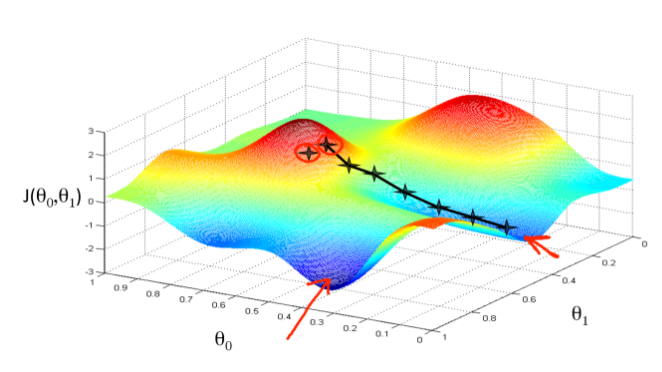
\includegraphics[height = 8cm, width = \textwidth]{Pictures/GradientDescent.png}
\caption{Beispiel des Gradient Descent Algorithmus an einer beliebigen Funktion}
\label{Gradient Descent}

\end{figure}
	        
\subsection{Verwendeten Platformen, Programmiersprachen und Bibliotheken}
Zur Datenerhebung per I²C wurde zwei weitgehend unterschiedliche Platformen verwendet. Zum einen wurde ein PICkit Serial Analyzer genutzt, um die Daten von einem Windows Rechner per Programmiersprache C# zu erheben. Dadurch, dass dieser Ansatz jedoch nur ein geringe Datenrate pro Sekunde erzielte, wurde stattdessen auf einen Raspberry Pi 4 gewechselt, welcher einer I²C Schnittstelle besitzt. Des Weiteren wurde für die Datenerfassung- und Verarbeitung die Sprache Python gewählt, da diese eine hohe Flexibilität bezüglich der Nutzbaren Bibliotheken mit sich bring. Das trainieren des Neuronalen Netzes erfolgt auf einem Windows Rechner mit der Maschine Learning Platoform Tensorflow, wobei Keras als High-Level API dient. Die graphische Visualisierung der Daten erfolgt ausschließlich per Pyplot library.
\end{flushleft}
